\documentclass[]{article}
\usepackage[spanish]{babel}
\usepackage{graphicx}
\usepackage[utf8]{inputenc}
\usepackage{fancyhdr}
\usepackage{lastpage}

\pagestyle{fancy}
\fancyhf{}
\rfoot{Page \thepage\hspace{1pt} de~\pageref{LastPage}}

\title{Practica 7}
\author{Guillermo Lopez Garcia}
\begin{document}
\maketitle

\textbf{Ejercicio 4.} \\

Los valores obtenidos en este ejercicio son exactamente los mismos
que los del anterior ejercicio, ya que, solo hace falta multiplicar
por 4 el valor obtenido y aproximamos a pi. Ya que, indirectamente,
lo que estamos haciendo con el método de montecarlo para la
función seno, es calcular 1/4 de pi. \\

\begin{figure}
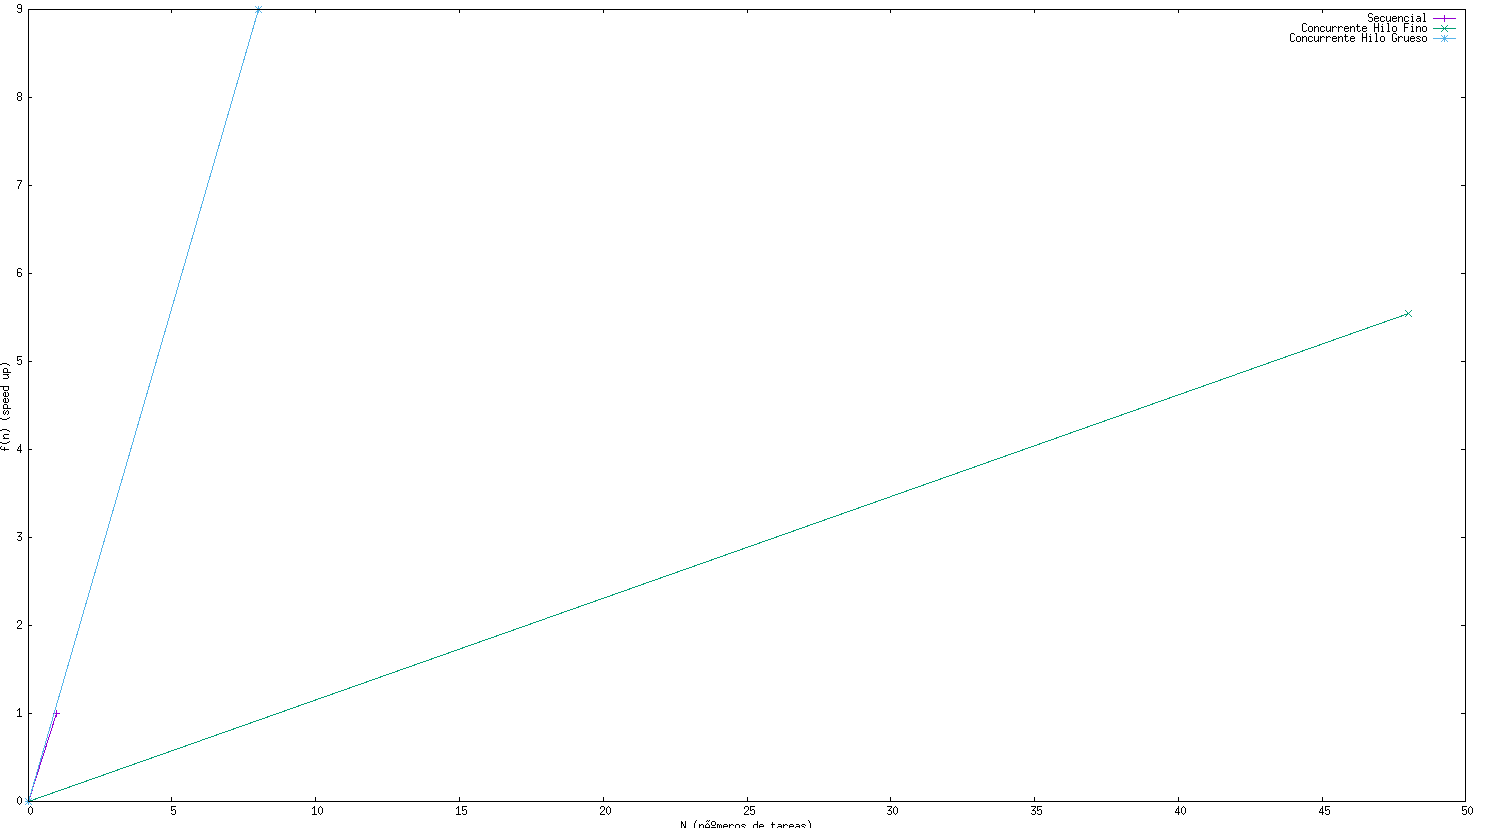
\includegraphics[width=\linewidth]{img.png}
\caption{Comparativa implementaciones concurrentes del método de montecarlo para pi.}
\label{fig:comp}
\end{figure}

\end{document}
